\documentclass[11pt]{report}
\usepackage{mathrsfs,graphicx}
\begin{document}

\noindent
George Weigt

\noindent
Homework \#3

\bigskip
\noindent
{\bf 1.} What is the Laplace transform of the following function?
\begin{center}
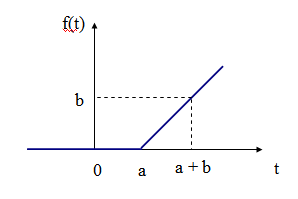
\includegraphics[scale=0.5]{images/211-1.png}
\end{center}

\bigskip
\noindent
The function $f(t)$ is the translated ramp function
$$f(t)=(t-a)\,1(t-a)$$
where $1(t-a)$ is the unit-step function (Ogata
p. 15.)
We have
$${\mathscr L}[f(t)]=e^{-as}{\mathscr L}[t]={e^{-as}\over s^2}$$

\bigskip
\noindent
{\bf 2.} What is the Laplace transform of the following function?
\begin{center}
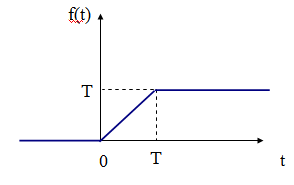
\includegraphics[scale=0.5]{images/211-2.png}
\end{center}

\bigskip
\noindent
The function $f(t)$ can be expressed as a ramp function minus a translated ramp
function.
$$f(t)=t\,u(t)-(t-T)\,u(t-T)$$
Hence
$${\mathscr L}[f(t)]={1\over s^2}-{e^{-Ts}\over s^2}$$

\newpage

\bigskip
\noindent
{\bf 3a.} Find the inverse Laplace transform of the following function.
$$F(s)={6s+3\over s^2}$$

\bigskip
\noindent
We have
$${\mathscr L}^{-1}[F(s)]={\mathscr L}^{-1}[6/s]
+{\mathscr L}^{-1}[3/s^2]=6+3t$$

\bigskip
\noindent
{\bf 3b.} Find the inverse Laplace transform of the following function.
$$F(s)={5s+2\over(s+1)(s+2)^2}$$

\bigskip
\noindent
By partial fraction expansion we have
$$F(s)=-{3\over s+1}+{3\over s+2}+{8\over(s+2)^2}$$
Hence
$${\mathscr L}^{-1}[F(s)]=-3e^{-t}+3e^{-2t}+8te^{-2t}$$

\end{document}
